\documentclass[bachelor, och, labwork]{shiza}

\usepackage{subfigure}
\usepackage{tikz,pgfplots}
\pgfplotsset{compat=1.5}
\usepackage{float}

\usepackage{titlesec}
\setcounter{secnumdepth}{4}
\titleformat{\paragraph}
{\normalfont\normalsize}{\theparagraph}{1em}{}
\titlespacing*{\paragraph}
{35.5pt}{3.25ex plus 1ex minus .2ex}{1.5ex plus .2ex}

\titleformat{\paragraph}[block]
{\hspace{1.25cm}\normalfont}
{\theparagraph}{1ex}{}
\titlespacing{\paragraph}
{0cm}{2ex plus 1ex minus .2ex}{.4ex plus.2ex}

% --------------------------------------------------------------------------%


\usepackage[T2A]{fontenc}
\usepackage[utf8]{inputenc}
\usepackage{graphicx}
\graphicspath{ {./images/} }
\usepackage{tempora}

\usepackage[sort,compress]{cite}
\usepackage{amsmath}
\usepackage{amssymb}
\usepackage{amsthm}
\usepackage{fancyvrb}
\usepackage{listings}
\usepackage{listingsutf8}
\usepackage{longtable}
\usepackage{array}
\usepackage[english,russian]{babel}

\usepackage[colorlinks=true]{hyperref}
\usepackage{url}

\usepackage{underscore}
\usepackage{setspace}
\usepackage{indentfirst} 
\usepackage{mathtools}
\usepackage{amsfonts}
\usepackage{enumitem}
\usepackage{tikz}
\usepackage{minted}

\newcommand{\eqdef}{\stackrel {\rm def}{=}}
\newcommand{\specialcell}[2][c]{%
\begin{tabular}[#1]{@{}c@{}}#2\end{tabular}}

\renewcommand\theFancyVerbLine{\small\arabic{FancyVerbLine}}


\begin{document}

% \chair{Кафедра теоретических основ компьютерной безопасности и криптографии}

\title{Умножение разреженных полиномов}

\course{3}

\group{331}

\department{факультета КНиИТ}

\napravlenie{10.05.01 "--- Компьютерная безопасность}

\author{Никитина Арсения Владимировича}

\satitle{доцент}

\saname{А. Н. Гамова}

\date{2022}

\maketitle

%-------------------------------------------------------------------------------
\tableofcontents

\intro
В данной работе будут рассмотрены принципы алгоритмов вычисления умножения 
разреженных полиномов, оценки работы алгоритмов в наилучшем и наихудшем случаях,
а также программная реализация алгоритмов. 

Арифметические операции, такие как умножение, над целыми числами и полиномами
лучше изучать в совокупности, так как многие алгоритмы, работающие с целыми 
числами по существу совпадают с алгоритмами, работающими с полиномами от одной
переменной. Это верно не только для таких операций, как умножение и деление, но
такое и для более сложно описываемых операций. Например, нахождение вычета
целого числа по модулю, задаваемому другим целым числом.


\section{Определение полинома}

Если $i$ - неотрицательное целое число то размер ($i$)=$\log i+1$. Если $p(x)$
- полином, то размер ($p$)=$CT(p) + 1$, где $CT(p)$ - степень полинома $p$, то
есть наибольшая степень переменной $x$ с нулевым коэффициентом.

Над целыми числами и полиномами моно выполнять приближенное деление. Если 
$a ~\text{и}~ b$ - два целых числа и $b \not= 0$, то найдется единственная пара
целых чисел $q ~\text{и}~ r$, для которых
\begin{enumerate}
    \item $a=bq + r$
    \item $r<b$,
\end{enumerate}

где $q ~\text{и}~ r$ -- соответственно частное и остаток от деления $a ~\text{и}~ b$.

Аналогично, если $a ~\text{и}~ b$ -- полиномы, причем $b$ отличен от постоянной,
то можно найти такие полиномы, что
\begin{enumerate}
    \item $a=bq+r$
    \item $CT(r)<CT(b)$
\end{enumerate}

\section{Разреженные полиномы}
Представляя полиномом от одной переменной в виде $\sum\limits_{i=0}^{n-1}{a_ix^i}$,
мы предполагали до сих пор, что он плотный, то есть отличны от нуля почти все 
его коэффициенты. Для многих приложений полезно предполагать, что полином
\textit{разрежен}, то есть число ненулевых коэффициентов много меньше его степени.
В такой ситуации логично представлять полином списком пар $(a_i, j_i)$, состоящих
из ненулевого коэффициента и соответствующего ему показателя степени переменной
$x$. 

\section{Умножение разреженных полиномов}

Наиболее оптимальная из известных стратегий умножения разреженных \\полиномов
состоит в том, что полином $\sum\limits_{i=1}^n{a_ix^{j_i}}$ задается списком пар:
\begin{center}$(a_1,j_1),...(a_n,j_n)$,\end{center}
где все $j_i$ различны и расположены в порядке убывания,
то есть $j_i>j_{i+1}$ для $1\leq i < n$. Чтобы умножить два полинома,
представленных таким образом, находим произведения пар и располагаем их по
величине показателей (по вторым компонентам пар), объединяя все члены с одинаковыми
показателями. Если это не делать, то придется расплачиваться ростом числа членов
с одинаковыми показателями. Поэтому по мере выполнения арифметических операций
сложность начнет значительно превосходить ту, которая была бы, если бы приведение
подобных членов выполнялась на каждом шаге.

\section{Умножение упорядоченных разряженных полиномов}

При умножении упорядоченных разряженных полиномов полиномов можно извлечь пользу
из их упорядоченности из того, что в одном из них может оказаться много больше
членов, чем в другом, чтобы максимально упростить упорядочение множества мономов
произведения.

Полиномы $f(x)=\sum\limits_{i=1}^m{a_ix^{j_i}} ~\text{и}~ g(x)=\sum\limits_{i=1}^n{b_jx^{k_i}}$
списками пар: 
\begin{center} $(a_1,j_1),...,(a_m,j_m),$\end{center}
\begin{center} $(b_1,k_1),...,(b_n,k_n),$\end{center}
где последовательности $j_1,...,j_m ~\text{и}~ k_1,...,k_n$ монотонно убывают

Полином $\sum\limits_{i=1}^p{c_ix^{l_i}} = f(x)g(x)$, представленный списком пар,
в котором последовательность $l_1,...,l_p$ монотонно убывает.

Предполагаем, что $m \ge n$. Затем:
\begin{enumerate}
    
    \item Строим последовательности $S_i,1 \le i \le n$, в которых $r$-й член,
    $1 \le r \le m ~\text{равен}~ (a_rb_i, j_r + k_i)$. Таким образом, $S_i$
    представляет произведение полинома $f(x)$ на $i$-й член полинома $g(x)$.

    \item Сливаем $S_{2i-1} ~\text{с}~ S_{2i} ~\text{для}~ 1\le i \le n/2$,
          приводя подобные члены. Затем попарно сливаем полученные 
          последовательности, приводя подобные члены, и повторяем процесс, пока 
          не получим одну упорядоченную последовательность.

\end{enumerate}

\section{Результаты тестирования программы}

        \begin{figure}[H]
            \centering
            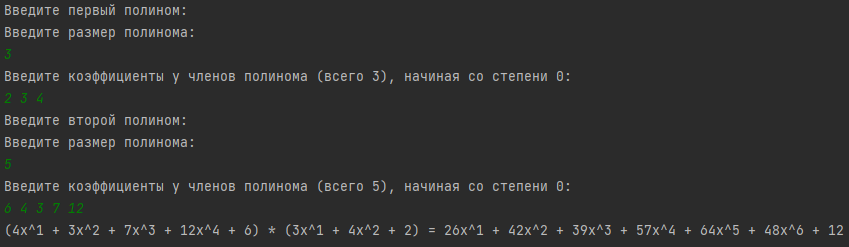
\includegraphics[width=0.8\textwidth]{2.png}
            \caption{}
        \end{figure}

\section{Программная реализация алгоритма}

\inputminted[linenos,breaklines=true, fontsize=\small, style=bw]{python}{3.py}



\section{Оценка работы алгоритма}

Алгоритм занимает $O(mn\log n)$ времени в предположении, что $m \ge n$:
\begin{enumerate}
    \item Первая часть алгоритма занимает $O(n,m)$ времени.
    \item Второй шаг алгоритма требуется повторить $\log n$ раз, и ясно, что при
          каждом выполнении процесса вся работа займет $O(mn)$ времени.
\end{enumerate}

\conclusion

В данной работе были рассмотрены основные определения полиномов и отличия
разреженных полиномов от плотных. Также был рассмотрен алгоритм построения
умножения разреженных полиномов и оценена скорость его работы. Затем алгоритм 
был реализован на практике. Перемножение двух разреженных полиномов можно 
асимптотически оценить в $O(mn\log n)$.

\end{document}